%%%%%%%%%%%%%%%%%%%%%%%%%%%%%%%%%%%%%%%%%%%%%%%%%%%%%%%%%%%%%%%%%%%%
%% I, the copyright holder of this work, release this work into the
%% public domain. This applies worldwide. In some countries this may
%% not be legally possible; if so: I grant anyone the right to use
%% this work for any purpose, without any conditions, unless such
%% conditions are required by law.
%%%%%%%%%%%%%%%%%%%%%%%%%%%%%%%%%%%%%%%%%%%%%%%%%%%%%%%%%%%%%%%%%%%%

\documentclass[
  digital, %% This option enables the default options for the
           %% digital version of a document. Replace with `printed`
           %% to enable the default options for the printed version
           %% of a document.
  notable,   %% Causes the coloring of tables. Replace with `notable`
           %% to restore plain tables.
  lof,     %% Prints the List of Figures. Replace with `nolof` to
           %% hide the List of Figures.
  lot,     %% Prints the List of Tables. Replace with `nolot` to
           %% hide the List of Tables.
  %% More options are listed in the user guide at
  %% <http://mirrors.ctan.org/macros/latex/contrib/fithesis/guide/mu/fi.pdf>.
]{fithesis3}
%% The following section sets up the locales used in the thesis.
\usepackage[resetfonts]{cmap} %% We need to load the T2A font encoding
\usepackage[T1,T2A]{fontenc}  %% to use the Cyrillic fonts with Russian texts.
\usepackage[
  main=english, %% By using `czech` or `slovak` as the main locale
                %% instead of `english`, you can typeset the thesis
                %% in either Czech or Slovak, respectively.
  german, russian, czech, slovak %% The additional keys allow
]{babel}        %% foreign texts to be typeset as follows:
%%
%%   \begin{otherlanguage}{german}  ... \end{otherlanguage}
%%   \begin{otherlanguage}{russian} ... \end{otherlanguage}
%%   \begin{otherlanguage}{czech}   ... \end{otherlanguage}
%%   \begin{otherlanguage}{slovak}  ... \end{otherlanguage}
%%
%% For non-Latin scripts, it may be necessary to load additional
%% fonts:
\usepackage{paratype}
\def\textrussian#1{{\usefont{T2A}{PTSerif-TLF}{m}{rm}#1}}
%%
%% The following section sets up the metadata of the thesis.
\thesissetup{
    date          = 2017/06/04, %\the\year/\the\month/\the\day,
    university    = mu,
    faculty       = fi,
    type          = bc,
    author        = Lenka Svetlovská,
    gender        = f,
    advisor       = {RNDr. Andriy Stetsko, Ph.D.},
    title         = {Security and cryptography in GO},
    TeXtitle      = {Security and cryptography in GO},
    keywords      = {keyword1, keyword2, ...},
    TeXkeywords   = {keyword1, keyword2, \ldots},
    bib           = example.bib,
}
\thesislong{abstract}{
    This is the abstract of my thesis, which can

    span multiple paragraphs.
}
\thesislong{thanks}{
    This is the acknowledgement for my thesis, which can

    span multiple paragraphs.
}
\usepackage{makeidx}      %% The `makeidx` package contains
\makeindex                %% helper commands for index typesetting.
%% These additional packages are used within the document:
\usepackage{paralist} %% Compact list environments
\usepackage{amsmath}  %% Mathematics
\usepackage{amsthm}
\usepackage{amsfonts}
\usepackage{url}      %% Hyperlinks
\usepackage{markdown} %% Lightweight Markup

%added usepackages
\usepackage{rotating} %rotate table?
%\newcommand*{\TitleInParbox}{\parbox[c]{0.3\linewidth}{\Title}}
\usepackage{longtable}
\usepackage{array}
\newcolumntype{P}[1]{>{\centering\arraybackslash}p{#1}}
\usepackage{enumitem}
\usepackage{graphicx,lipsum,wrapfig}
\usepackage{footnote}
\usepackage{listings}

\usepackage{color}

%New colors defined below
\definecolor{codegreen}{rgb}{0,0.6,0}
\definecolor{codegray}{rgb}{0.5,0.5,0.5}
\definecolor{codepurple}{rgb}{0.58,0,0.82}
\definecolor{backcolour}{rgb}{0.95,0.95,0.92}

%Code listing style named "mystyle"
\lstdefinestyle{mystyle}{
  backgroundcolor=\color{backcolour},   commentstyle=\color{codegreen},
  %keywordstyle=\color{magenta},
  numberstyle=\tiny\color{codegray},
  %stringstyle=\color{codepurple},
  basicstyle=\footnotesize,
  breakatwhitespace=false,         
  breaklines=true,                 
  captionpos=b,                    
  keepspaces=true,                 
  numbers=left,                    
  numbersep=5pt,                  
  showspaces=false,                
  showstringspaces=false,
  showtabs=false,                  
  tabsize=2
}

%"mystyle" code listing set
\lstset{style=mystyle}




\begin{document}
\chapter{Introduction}


\chapter{Basic Terms}
In this section, I define the basic terms which are necessary to an understanding of the text 
presented in the following chapters. First I explain the symmetric and asymmetric 
cryptography, X.509 certificates, protocols SSL and TLS. Finally, I describe TLS\_PSK, which 
is indispensable for working with ......

\section{Cryptography}
Cryptography is the study of mathematical techniques related to aspects of information
security such as confidentiality, data integrity, entity authentication, and data origin
authentication \cite{menezes1996handbook}. %Together with cryptanalysis, which is engaged in deciphering codes without the secret knowledge key, is the part of science called cryptology.
%\vskip 0.2in
%Already in the nineteenth century, Auguste Kerckhoffs formulated the principle which has been true in cryptography today. Safety of cryptosystem must not depend on the secrecy of the algorithm. It must be publicly known, and security must depend only on the secret key \cite{menezes1996handbook}. 
Today we talk about computer security which consists in the fact that the attacker does not 
have enough computational strength and time to decode the cipher. 
%Discrete logarithm and factorization of large numbers belong to the issues for which there is no effective algorithm today.
%\vskip 0.2in
We can divide cryptography base on the type of keys into three parts. They are symmetric 
cryptography, asymmetric cryptography, and other primitives %, for example, hash functions, one-way permutation or random number generators
\cite{menezes1996handbook}.

%%OBRAZOK
%\begin{figure}[th]
%	\centering
%	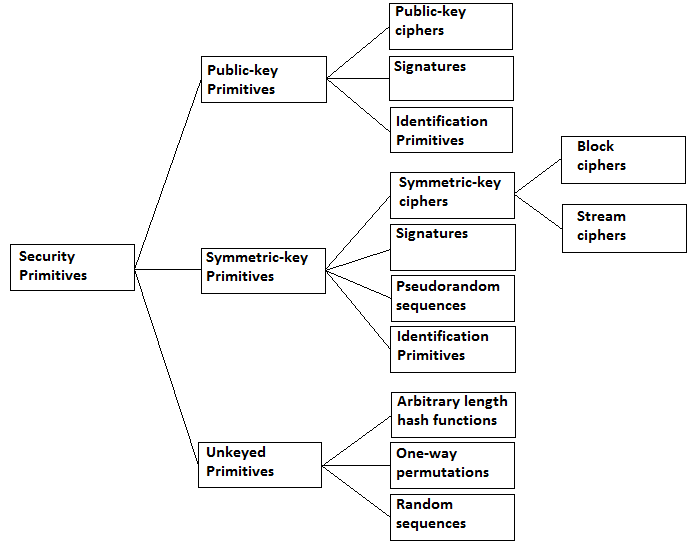
\includegraphics[width=0.82\textwidth]{securityPrimitives}
%	\caption{A taxonomy of cryptographic primitives}
%	\label{fig:secPrim}
%\end{figure}
%%info handbook strana 23

\subsection{Symmetric Cryptography}
%The beginnings of symmetric cryptography date back to around 2000 BC.\cite{singh2011code}. 
Symmetric encryption, as the name suggests, means that the encryption and decryption of 
plaintext are based on sharing a together secret - keys. The secret key could be a number, a 
word or just string of random letters. %This problem, however, stems directly from the provisions of a mystery. The problem of secure transfer of the message, in this case, is only converted to the issue of secure transmission of secret keys. This situation we can solve by other means, such as personal meetings or any infrastructure provided key distribution. Globally, all similar approaches proved to be unsuitable \cite{singh2011code}.
%\vskip 0.2in 

Symmetric ciphers could be divided into block and stream. Stream ciphers encrypt each 
character of plaintext separately, usually one bit. Block ciphers encrypt plaintext into 
blocks with fixed bit length \textit{n}. %Messages, which have more than \textit{n} bits, are separated into \textit{n}-bit blocks and then they are encrypted. 
%We distinguish several basic modes, such as ECB (Electronic Codebook), CBC (Cipher Block Chaining), CFB (Cipher Feedback) and OFB (Output Feedback), CTR (Counter Mode) \cite{piper2006kryptografie}.
%Stream ciphers are typically faster and easier for hardware implementation. They are often used in telecommunication applications, where we can use a very limited buffer. Their using is also advantageous in environment where is a significant probability of errors in the transmission because there is no propagation of this error to other data. In turn, block ciphers can perform the function Message Authentication Code (MAC) or hash functions.

The main disadvantage of symmetric cryptography is the necessity of a large number of keys 
and need of their distribution. For example, for together communication \textit{n} operators 
need to have \[ \frac{n * (n - 1)}{2}\] keys. It means that for the encrypted communications 
of mid-size company with 50 employees, it would need to share 1225 different keys. 

On the other hand, the advantage is the low computational complexity of symmetric ciphers. 
Their using is also useful in cases where the encrypted data are not sent anywhere, for 
example, to protect files on a personal computer.
 
\subsection{Asymmetric Cryptography}
%Unlike symmetric cryptography, asymmetric cryptography is very young. Its origins could be found in 1977 when the RSA cryptosystem was created based on the impossibility of effectively factorize of large numbers. In fact, the beginning of asymmetric cryptography was established a few years earlier by Clifford Cocks. His research, however, was still kept secret until recently \cite{singh2011code}.
%\vskip0.2in
Asymmetric cryptography allows data encryption and particularly the implementation of the 
digital signature. Each entity has two keys. The first is the private key that is used to 
decrypt a message or create a digital signature. It must be kept secret. The second key is 
public which is used for encryption and authentication of the digital signature. Of course, 
there is impossible to derive the private key from the public key \cite{dostalek2016velky}.
%Asymmetric cryptography, itself, does not solve the authenticity of the public key. It is necessary to decide whether the given public key belongs to given entity. The solution of this problem is the infrastructure of the public key \cite{dostalek2016velky} which is nowadays the most widespread means of ensuring the credibility of the digital signature.

The main advantages of asymmetric cryptography are mainly a smaller number of keys than 
symmetric cryptography. If each entity has one public and one private key, it means that for 
\textit{n} entities are needed \textit{2n} keys. In the same situation as in the previous 
example, a company of 50 employees would need to ensure the safety of 100 keys, which is 
substantially less than 1225.
%\vskip0.2in

The biggest disadvantage of asymmetric cryptography is its slowness compared with symmetric 
cryptography. Therefore, they are most often used together, while the text is encrypted with a 
random symmetric encryption key. The key is encrypted using asymmetric ciphers. In the case of 
a digital signature, the first is created the fixed length hash of the message and then it is 
signed using asymmetric cryptography.

\subsection{Hash Function}
Hash functions are one of the basic elements of modern cryptography, often called one-way 
hash function.
%\vskip0.2in

Hash functions are effectively designed display binary strings unlimited length to binary 
strings a fixed length, called hash value. For a perfect hash function that has \textit{n}-bit 
hash value, there is a chance that a randomly selected string will be displayed on specific 
hash value $2^{-n}$. The basic idea of hash functions is that the hash value should serve as a 
representative of the input string. Hash function suitable for use in cryptography is usually 
chosen so that it is computationally very difficult find two different input strings that have 
the same hash value. If it succeeds in these two find strings, we say that we found a 
collision. 
Likewise, it should be computationally very difficult to find for a hash value corresponding 
to the input string. Using hash functions are used frequently to check the integrity of data 
and for digital signing of data \cite{piper2006kryptografie}.

ITEMIZE

\section{Certificate}
Certificate is digitally signed data structure whose foundation includes a public key of
certificate owner. There are some standards of structure the certificate (X.509, EDI, WAP, 
etc.). The Internet is based on standard X.509 version 3, which issued the ITU. For the needs 
of the Internet, there is created an Internet profile of X.509 in the relevant RFC. Current 
Internet profile certificate is standard RFC-5280 \cite{dostalek2016velky}.

\subsection{Standard X.509}
Standard X.509 was originally designed as an authentication framework for X.500 
directories \cite{schmeh2006cryptography}. They have a hierarchical structure and the 
individual attributes can be assigned to individual computers of companies or individual 
printers. That is, each entity can be clearly identified, and each can have its private and 
public key. The proposal envisages the hierarchical structure of certificate authorities. 
Certificate X.509, see Figure \ref{fig:certificate}.
\vskip 0.1in
The first version of the X.509 standard was already appeared in 1988 as the first proposal for 
PKI \cite{schmeh2006cryptography}. The first version was very simple and today is already 
inadequate. It contained only 7 fields:
\vskip 0.1in
\begin{itemize}[leftmargin=2em,rightmargin=1em,itemsep=0.75\parskip,parsep=0em,topsep=0em,partopsep=0em]
\item certificate version;
\item certificate series number;
\item algorithm which signed certificate;
\item name of certification authority which certificate released;
\item identity of certificate owner;
\item public key of certificate owner;
\item certificate validity.
\end{itemize}
\vskip 0.1in
The second version was introduced five years later in 1993 and brought only minimal changes. 
The second version did not solve the problems associated with the first version. Fields which 
was needed in this version, still missing \cite{schmeh2006cryptography}. It contained only two 
new fields:
\vskip 0.1in
\begin{itemize}[leftmargin=2em,rightmargin=1em,itemsep=0.75\parskip,parsep=0em,topsep=0em,partopsep=0em]
\item unique identifier of the certificate owner;
\item unique identifier of the certification authority.
\end{itemize}
\vskip 0.1in
The third version was introduced in 1996. Its biggest and most important benefit is to support 
the expansion. It is defined a syntax that allows you to create custom certificate extension. 
It eliminates the major shortcomings of the two previous versions, but then appears some 
incompatibility. 

\begin{figure}[th]
	\centering
	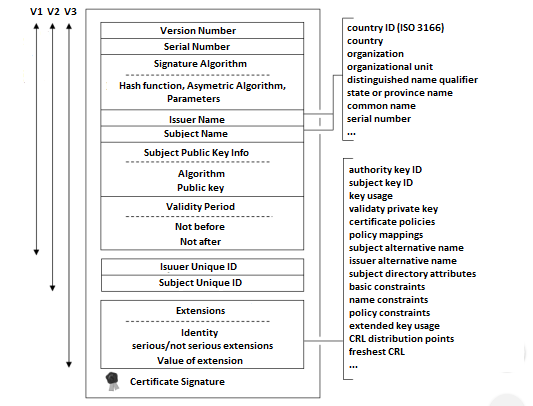
\includegraphics[width=1\textwidth]{certificate}
	\caption{Structure X.509 Certificate}
	\label{fig:certificate}
\end{figure}
%% Zdroj info o obrazku:
% @techreport{housley2002internet,
%   title={Internet X. 509 public key infrastructure certificate and % certificate revocation list (CRL) profile},
%   author={Housley, Russell and Polk, William and Ford, Warwick and Solo, David},
%  year={2002}
% }

%To the protocols which mostly use X.509 certificates, belongs primarily SSL, TLS.

\subsection{Certificate Authority}
Certification Authority (CA) is an independent third party that issues certificates. 

In other words, the CA is an institution which inspects the certificate request and issues 
certificates whose validity is verifiable using the responsive public key. The CA also takes 
care of archiving and distribution of certificates checks their validity and ensures their 
revocation. To the CA is truly credible, it must be impartial and, if it is possible, it 
should be subordinate any higher CA. Subordination means that it identifies using a 
certificate signed by the certification authority higher level \cite{dostalek2016velky}.

Root CA, certification authorities at the highest level, uses the certificate signed by 
themselves (self-signed certificate).

\subsection{Self-signed Certificate}
The self-signed certificate is a certificate which the applicant gives by itself. The 
self-signed certificate has the same data structure as a certificate issues by CA. This 
certificate is recognized according to identical item Subject and item Issuer.

Creating self-signed certificate is not easy. To create certificate request we need to fill 
same items, which we do not know. For example, serial number, certificate validity, etc.

As proof of the private key possession by the user, the self-signed certificate uses a 
digital signature certificate which was made by the private key belonging to the public key 
in the certificate. Verification of the signature is carried out through a public key in the 
actual certificate \cite{dostalek2016velky}.

Self-signed certificate is used by software internally. While the applicant generates CSR to 
be issued by the CA, the public key must be kept by the applicants. In this case, the public 
key is often maintained like a self-signed certificate. Subsequently it is rewritten by the 
certificate.

\subsection{Formats PEM and DER}
The PEM (Privacy Enhanced Mail) is a Base64 encoded DER certificate. It is designed 
to be safe for inclusion in ASCII or even rich-text documents. This means that we can simple 
copy and paste the content of a pem file to another document and back. Following is a sample 
PEM file containing a private key and a certificate \ref{fig:vzorPEM-DER}.

\begin{figure}[th]
	\centering
	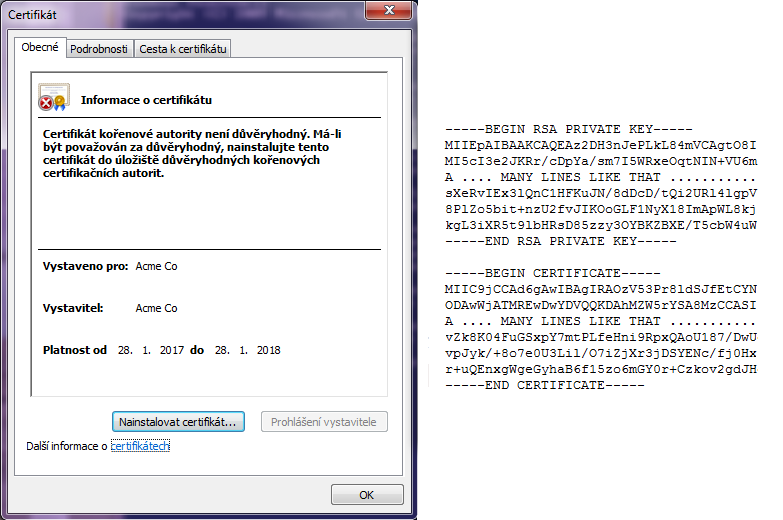
\includegraphics[width=1\textwidth]{pem-der}
	\caption{A sample example of DER and PEM file}
	\label{fig:vzorPEM-DER}
\end{figure}

A certificate or key must start with header and the number of dashes is meaningful, and must 
be correct. A single PEM file can contain a number of certificates and a key, for example, a 
single file with public certificate, intermediate certificate, root certificate or private key 
\cite{howToSsl}.

The DER (Distinguished Encoding Rules) is a binary form of ASCII PEM format 
certificate. All types of certificates and private keys can be encoded in DER format, its 
information is stored in the binary DER for ASN.1 and applications providing RSA, SSL and TLS 
should handle DER encoding to read in the information \cite{bakker_2014}.

\subsection{Certificate Signing Request}
The certificate authority must fill individual items of the certificate duly before it signs 
the result digitally. The certificate applicant can apply in two ways: submit a data 
structure called a certificate request or not so \cite{dostalek2016velky}.

The certificate request should include:
\begin{itemize}[leftmargin=2em,rightmargin=1em,itemsep=0.75\parskip,parsep=0em,topsep=0em,partopsep=0em]
\item Applicant ID
\item The public key
\item Evidence of the possession of the private key
\item Other information that the user wishes to insert certificate
\item May contain evidence of the generation of paired data
\item Data necessary for billing (in case issuance of certificates is paid)
\item Passwords for communication with CA:
  \begin{itemize}[leftmargin=2em,rightmargin=1em,itemsep=0.75\parskip,parsep=0em,topsep=0em,partopsep=0em]
  \item One-time password for issuing the certificate
  \item One-time password for certificate revocation
  \item Permanent password for personal (non-electronic) communication between user and CA
  \item Phrase (in case losing every passwords) 
  \end{itemize}
\end{itemize} 

\subsection{PROCESY - podpisovanie a cert. exchange}


\section{Protocols SSL and TLS}
Protocols SSL and TLS are used for secure communications between client and server. They 
create a framework for the use of encryption and hash functions.

SSL was developed by Netscape Communications which published three versions. The first version 
was only a test, the second has been used in practice. However, it still contained security 
vulnerabilities, the most important was susceptibility to attack \textit{man in the middle}. %zdroj?? https://scholar.google.sk/scholar?q=Security+Technologies+for+the+World+Wide+Web&btnG=&hl=sk&as_sdt=0%2C5 
The third version was introduced in 1996 and its specification could be found in the document 
\textit{The SSL Protocol Version 3.0} \cite{freier2011secure}. Of this version was created TLS 
protocol which is currently the most widespread and supported \cite{oppliger2003security}. 
There are three versions which have only minimal differences.

Protocol SSL/TLS provides authentication of the two communicating parties by using asymmetric 
encryption, message integrity by using MAC and confidentiality by encrypting all 
communications by selected symmetric cipher.

Protocol SSL/TLS is located between the application and the transport layer reference ISO/OSI 
model and consists of two main parts. They are \textit{The Record Layer Protocol} (RLP) and 
\textit{Handshake Protocol} (HP). %Part of HP are two auxiliary protocols - \textit{Change Cipher Specification Protocol} (CCSP) and \textit{Alert Protocol} (AP) \cite{oppliger2003security}.

\textit{Record Layer Protocol} processes application data, performs fragmentation, compression 
and data encryption. On the other hand, it decrypts the data again and verifies the checksums. 
RLP protocol does not care about the type of encryption algorithm or encryption key setting. 
This information is from HP.

\textit{Handshake Protocol} is activated immediately after establishment the connection and 
provides identification of communicating parties, provision of cryptographic algorithms, 
compression algorithms and other attributes. Then it creates \textit{a master secret} from 
which are derived encryption keys, initiation vectors and the MAC. The process of the protocol 
is:
\vskip0.1in
\begin{enumerate}
\item The client wants to connect to the server and sends \textit{ClientHello}, which contains 
the highest number of version supported by SSL/TLS, the number of session (it is empty if it 
is a new session), the list of supported ciphers and compression methods and a random number.
\item The client waits for a response in the form of a report \textit{ServerHello}, which will 
contain the highest number of versions of SSL/TLS, which is supported by server and client. It 
will also contain encryption and compression method, which are selected from the list received 
in step one, a random number and its public key certificate (the server can also request 
authentication client).
\item The client verifies the server certificate, if all ciphers are satisfied. Next, he sends 
a request to server to exchange keys. At the end the server and client share a common 48 bits 
\textit{premaster secret}. \textit{The master secret} is derived from it. Then of the master 
secret and random numbers \textit{ClientHello ServerHello} are derived two session keys to 
encrypt messages and two MAC initiation vectors for use symmetric cipher in CBC mode. 
\item The client sends a confirmation selected ciphers. From this moment, the communication 
has been encrypted and the client sends a message that ends with this phase. In case the 
server required the client authentication, it has been carried out in this step. Finally, the 
server sends a confirmation used ciphers and message about the completion of this phase, 
thereby HP ends.
\end{enumerate}

%\textit{Change Cipher Specification Protocol} is a simple protocol that contains only a single message. It says there was the change of the encryption parameters and now only new ones will be used. It could be also called after the end of the initial phase.

%\textit{Alert protocol} provides the transmission of warning in case of any problem in communication - it contains an array of warning severity and description of the problem.
 
The used algorithms:
\begin{itemize}[leftmargin=2em,rightmargin=1em,itemsep=0.75\parskip,parsep=0em,topsep=0em,partopsep=0em]
\item key exchange: RSA, Diffie-Hellman, ECDH;
\item stream symmetric ciphers: RC4 with key length of 40-120 bits;
\item block symmetric ciphers: DES, DES40, 3DES, IDEA;
\item hashing algorithms: MD5, SHA.
\end{itemize}
\vskip0.1in
TLS uses public key certificates for authentication. To establish a TLS connection are used 
symmetric keys (later called pre-shared keys or PSKs), shared in advance among the 
communicating parties \cite{eronen2005pre}.

\subsection{PSK Key Exchange Algorithm}
The cipher suites with PSK key exchange algorithm, use only symmetric key algorithms and are 
thus especially suitable for performance-constrained environments where both ends of the 
connection can be controlled. The cipher suites are intended for a rather limited set of 
applications, usually involving only a very small number of clients and servers.

%\begin{figure}[th]
%	\centering
%  	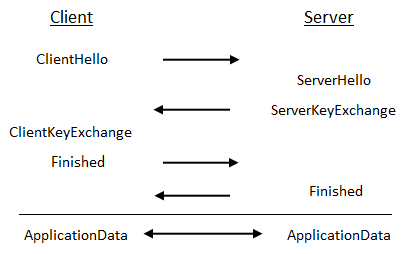
\includegraphics[width=0.5\textwidth]{psk}
%   \caption{TLS PSK}
%   \label{fig:psk}
%\end{figure}

\begin{wrapfigure}{r}{0.5\textwidth}
	\vspace{-20pt}
    \begin{center}
   		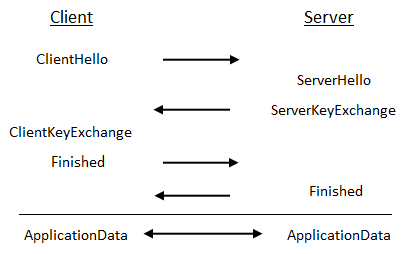
\includegraphics[width=0.5\textwidth]{psk}
	\end{center}
    \vspace{-20pt}
    \caption{TLS PSK}
    \vspace{-10pt}
	%\label{fig:psk}
\end{wrapfigure}

The client indicates its willingness to use pre-shared key authentication by including one or 
more PSK ciphersuites in \textit{the ClientHello message}. If the TLS server also wants to use 
pre-shared keys, it selects one of the PSK ciphersuites, places the selected ciphersuite in 
\textit{the ServerHello message}, and can includes \textit{ServerKeyExchange message}. If 
\textit{ServerKeyExchange message} is included depends on the server provides to help the 
client in selecting which identity to use. The server can provide a "PSK identity hint" in 
\textit{the ServerKeyExchange message}. The client indicates which key to use by including a 
"PSK identity" in \textit{the ClientKeyExchange message}. If no hint is provided, \textit{the 
ServerKeyExchange message} is omitted. Both clients and servers may have pre-shared keys with 
several different parties. The Certificate and CertificateRequest payloads are omitted from 
the response.

The TLS handshake is authenticated using \textit{the Finished messages} as usual. If the 
server does not recognize the PSK identity, it may respond with an 
\textit{unknown\_psk\_identity alert message}.  Alternatively, if the server wishes to hide 
the fact that the PSK identity was not known, it may continue the protocol as if the PSK 
identity existed but the key was incorrect: that is, respond with \textit{a decrypt\_error 
alert} \cite{eronen2005pre}. 

\chapter{Language GO}
Go is a programming language developed at \textit{Google} in year 2007 and announced in 
November 2009. Many companies have started using Go because of its performance, simplicity, 
ease of use and powerful tooling. Go programming language is a statically-typed language with 
advanced features and a clean syntax \cite{doxsey2016introducing}. It combines the performance 
and security benefits associated with using a compiled language like \textit{C++} with the 
speed of a dynamic language like \textit{Python}. It provides:
\vskip0.1in
\begin{itemize}[leftmargin=2em,rightmargin=1em,itemsep=0.75\parskip,parsep=0em,topsep=0em,partopsep=0em]
\item garbage collector - memory is cleaned up automatically when nothing refers to it 
anymore,
\item fast compilation time - through effective work with addictions individual parts of the 
program and simple grammar,
\item light-weight processes (via go-routines), channels,
\item a rich standard library,
\item easy testing - incorporated directly into the core language,
\item one of the best documentation - a clear and full of examples.
\end{itemize}
\vskip0.1in

Go excluded some features intentionally to keep language simple and concise. There is no 
support for type inheritance, method or operator overloading, circular dependencies among 
packages, pointer arithmetic, assertions nor for generic programming.

\section{Packages}
In Go, source files are organized into system directories called packages. To  develop 
software applications, writing maintainable and reusable pieces of code is very important. Go 
provides the modularity and code reusability through it’s package system. Go encourages 
programmers to write small pieces of software components through packages, and compose their  
applications with these small packages.

The packages from the standard library are available at the “pkg” subdirectory of the GOROOT 
directory. When we install Go, an environment variable GOROOT will be automatically added to 
our system for specifying the Go installer directory. The Go developer community is very 
enthusiastic for developing third-party Go packages. When you develop Go applications, you can 
leverage these third-party Go packages \cite{stack_2014}.

When programmers develop executable programs, they will use the package “main” for making the 
package as an executable program. The package “main” tells the Go compiler that the package 
should compile as an executable program instead of a shared library. When programmers build 
shared libraries, they will not have any main package and main function in the package.

To download third-party Go packages is used command: 
\begin{lstlisting}
go get example/exampleLib
\end{lstlisting}
After installing the exampleLib, put the import statement in programs for reusing the code, as 
shown below:
\begin{lstlisting}
package db
import (
	"example/exampleLib"
	"example/exampleLib/sub"
)
func init {
	// initialization code here    
}
\end{lstlisting}
To install third-party Go packages is used command: 
\begin{lstlisting}
go install
\end{lstlisting}
The go install command will build the package “sub” which will be available at the pkg 
subdirectory of GOPATH.
\begin{lstlisting}
package main
import (
	"fmt"
	"example/exampleLib/sub"
)
func main() {
    sub.Add("dr","Dart")
    fmt.Println(sub.Get("dr"))
    // code here    
}
\end{lstlisting}

\subsection{Crypto}
Package crypto collects common cryptographic constants.

\begin{table}[th]
\begin{tabular}{|p{1.5cm} p{10.5cm}|}
\hline
Crypto & Description \\
\hline
aes & implements AES encryption (formerly Rijndael), as defined in U.S. Federal Information Processing Standards Publication 197. \\
cipher & implements standard block cipher modes that can be wrapped around low-level block cipher implementations. \\
des &  implements the Data Encryption Standard (DES) and the Triple Data Encryption Algorithm (TDEA) as defined in U.S. Federal Information Processing Standards Publication 46-3. \\
dsa &  implements the Digital Signature Algorithm, as defined in FIPS 186-3.implements the Elliptic Curve Digital Signature Algorithm, as defined in FIPS 186-3.\\
esdsa & implements the Elliptic Curve Digital Signature Algorithm, as defined in FIPS 186-3. \\
elliptic &  implements several standard elliptic curves over prime fields. \\
hmac & implements the Keyed-Hash Message Authentication Code (HMAC) as defined in U.S. Federal Information Processing Standards Publication 198. \\
md5 & implements the MD5 hash algorithm as defined in RFC 1321. \\
rand & implements a cryptographically secure pseudorandom number generator.\\
rc4 &  implements RC4 encryption, as defined in Bruce Schneier's Applied Cryptography.\\
rsa & implements RSA encryption as specified in PKCS\#1. \\
sha1 & implements the SHA1 hash algorithm as defined in RFC 3174.\\
sha256 & implements the SHA224 and SHA256 hash algorithms as defined in FIPS 180-4. \\
sha512 & implements the SHA-384, SHA-512, SHA-512/224, and SHA-512/256 hash algorithms as defined in FIPS 180-4.\\
subtle & implements functions that are often useful in cryptographic code but require careful thought to use correctly.\\
tls & partially implements TLS 1.2, as specified in RFC 5246. \\
x509 & parses X.509-encoded keys and certificates. It contains package pkix which contains shared, low level structures used for ASN.1 parsing and serialization of X.509 certificates, CRL and OCSP. \\ 
\hline
\end{tabular}
\caption{Table of crypto package created by golang} 
\label{table:crypto} 
\end{table}
% ZDROJ: https://golang.org/pkg/

\subsection{Encoding}
Package encoding defines interfaces shared by other packages that convert data to and from 
byte-level and textual representations.

\begin{table}[th]
\begin{tabular}{|p{1.5cm} p{10.5cm}|}
\hline
Encoding & Description \\
\hline
ascii85 & implements the ascii85 data encoding as used in the btoa tool and Adobe's PostScript and PDF document formats. \\
asn1 & implements parsing of DER-encoded ASN.1 data structures, as defined in ITU-T Rec X.690. \\
base32 & implements base32 encoding as specified by RFC 4648. \\
base64 & implements base64 encoding as specified by RFC 4648. \\
biary & implements simple translation between numbers and byte sequences and encoding and decoding of variants. \\
csv & reads and writes comma-separated values (CSV) files. \\
gob & manages streams of gobs - binary values exchanged between an Encoder (transmitter) and a Decoder (receiver). \\
hex & implements hexadecimal encoding and decoding. \\
json & implements encoding and decoding of JSON as defined in RFC 4627. \\
pem & implements the PEM data encoding, which originated in Privacy Enhanced Mail. \\
xml & implements a simple XML 1.0 parser that understands XML name spaces. \\
\hline
\end{tabular}
\caption{Table of encoding package created by golang} 
\label{table:encoding} 
\end{table}
% ZDROJ: https://golang.org/pkg/

\subsection{Hash}
Package hash provides interfaces for hash functions.

\begin{table}[th]
\begin{tabular}{|p{1.5cm} p{10.5cm}|}
\hline
Hash & Desription \\
\hline
adler32 & implements the Adler-32 checksum. \\
crc32 & implements the 32-bit cyclic redundancy check, or CRC-32, checksum. \\
crc64 & implements the 64-bit cyclic redundancy check, or CRC-64, checksum. \\
fnv & implements FNV-1 and FNV-1a, non-cryptographic hash functions created by Glenn Fowler, Landon Curt Noll, and Phong Vo. \\
\hline
\end{tabular}
\caption{Table of hash package created by golang} 
\label{table:hash} 
\end{table}
% ZDROJ: https://golang.org/pkg/

\chapter{Analysis}
It was necessary to examine features of language GO related safety and cryptography, analyze 
libraries which GO contains and also search for available third-party libraries. This chapter 
contains the overview, evaluate and compare existing cryptographic liberates base on their 
measures and next base on expansion measures important for implementation.

Table \ref{table:analysis} shows analyzed Go package Crypto created by Golang and other Go 
packages created by third-parties. Individually items mean:
\vskip0.1in
\begin{itemize}[leftmargin=2em,rightmargin=1em,itemsep=0.75\parskip,parsep=0em,topsep=0em,partopsep=0em]
\item Name - name of founder and package.
\item Cryptographic functions - support cryptographic functions, such as symmetric encryption, asymmetric encryption and hash functions (all/sym/asym/hash/unknown).
\item Start of project - a year of creating project.
\item Is still opened - contributors still work on the project (Yes/No).
\item Issue tracker system - support of solving bugs, feature requests, tracking todos, and more (Yes/No).
\item Documentation accessibility - assessed on a scale of 0-5 (5 is the highest).
\item Downloads - number of downloads. In case the package is saved on \textit{https://github.com/}, the information about downloads presents value of Fork. Downloads of package Crypto created by Golang is unknown, this package is automatically installed with installing program Go.  
\item License - availability of licenses for free (Yes/Payment). The payment indicates the amount of payment per some period. This case did not occur.
\end{itemize}
\vskip0.1in

\begin{center}
\begin{longtable}[th]{|P{1.6cm}P{1cm}P{1cm}P{1cm}P{1.3cm}P{1.3cm}P{1.2cm}P{1.1cm}|}
\caption{Table of cryptographic libraries in Go} \label{table:analysis} \\

\hline Name & Crypto. functions & Start of project & Is still opened & Issue tracker system & Doc. accessability & Down-loads & License\\ \hline 
\endfirsthead

\multicolumn{8}{c}%
{{\tablename\ \thetable{} -- continued from previous page}} \\
\hline Name & Crypto. functions & Start of project & Is still opened & Issue tracker system & Doc. accessability & Down-loads & License \\ \hline 
\endhead

\hline \multicolumn{8}{|r|}{{Continued on next page}} \\ \hline
\endfoot

\hline \hline
\endlastfoot

golang/ crypto & all & 2009 & Y & Y & 5 & - & Y\\ 
%go-lang. cat-v.org/ pure-go-libs & N & \footnote{Page ceased updating in October, 2012} & & & & & Y \\ 
%golang libs.com category cryptography & Y & not all & 2012-2016 & some & & & \\
%golang libs.com category security & Y & not all & 2013-2016 & some & & & \\
ory-am/ fosite & asym, hash & 2015 & Y & Y & 4 & 39 & Y \\
square/ go-jose & asym, sym & 2014 & Y & Y & 4 & 70 & Y \\
Shopify/ ejson & hash & 2014 & Y & Y & 3 & 22 & Y \\
mitchellh/ go-mruby & asym & 2014 & Y & Y & 4 & 19 & Y \\
Sermo Digital/ jose & all & 2015 & Y & Y & 4 & 28 & Y \\
mozilla/ tls-observatory & hash & 2014 & Y & Y & 4 & 31 & Y \\
square/ certigo & hash & 2016 & Y & Y & 3 & 12 & Y \\
docker/ libtrust & all & 2014 & N & Y & 4 & 26 & Y \\
dedis/ crypto & sym, hash & 2010 & Y & Y & 4 & 17 & Y \\
dchest/ blake2b & hash & 2012 & N & Y & 4 & 6 & Y \\
enceve/ crypto & hash & 2016 & N & Y & 4 & 1 & Y \\
go-libp2p-crypto & all & 2015 & Y & Y & 4 & 5 & Y \\ 
dchest/ blake2s & hash & 2012 & N & N & 3 & 3 & Y \\
benburkert/ openpgp & sym, hash & 2012 & N & N & 3 & 0 & Y \\
minio/ sha256-simd & hash & 2016 & Y & Y & 3 & 14 & Y \\
avelino/ awesome-go & un-known & 2014 & Y & Y & 2 & 2287 & Y \\
ethereum/ go-ethereum & all & 2013 & Y & Y & 4 & 1028 & Y \\
chain/ chain & hash & 2015 & Y & Y & 4 & 113 & Y \\
lightning network/lnd & sym, hash & 2015 & Y & Y & 4 & 50 & Y \\
square/ go-jose & asym, hash & 2014 & Y & Y & 4 & 70 & Y \\
dgrijalva/ jwt-go & asym, hash & 2012 & Y & Y & 4 & 226 & Y \\
golang/ oauth2 & asym, hash & 2014 & Y & Y & 4 & 279 & Y  
\end{longtable}
\end{center}
%%  Zdroje k tabulke:
%%% https://golanglibs.com/top?q=security
%%% https://golanglibs.com/category/cryptography?sort=top
%%% http://go-lang.cat-v.org/pure-go-libs
%%% https://godoc.org/golang.org/x/crypto
%%% https://golang.org/pkg/
%%% ?

The table \ref{table:analysis} was created on the base of information available on 
following websites \cite{security-golibrariesAndApps} \cite{cryptography-golibrariesAndApps} \cite{crypto-godoc} \cite{packages-thegoprogramminglanguage}. The 
table does not contain packages which do not support any cryptographic functions. Also, 
the table does not contain information from untrusted sources. During the analysis, I 
discovered sources which are not actual or supported \cite{puregolibs}.

The next step of analysis was select the libraries which fulfill the requirements. The important 
parameters were the support of all cryptographic functions, the topicality of project, the 
approach to solving problems and no payment license. In the table \ref{table:analysis2}, 
there are shown four libraries and compared to the base of the other measures:
\vskip0.1in
\begin{itemize}[leftmargin=2em,rightmargin=1em,itemsep=0.75\parskip,parsep=0em,topsep=0em,partopsep=0em]
\item Crypto. key - possibilities for generation of cryptographic keys (Yes/No),
\item X.509 Certificates - work with X.509 certificates (generation of self-signed certificates, support for certificate signing requests, support for different formats and extensions) (Yes/No),
\item SSL/TLS - support of higher level protocols such as SSL/TLS (Yes/No),
\item Use go lang crypto - dependence on Crypto package created by Golang (Yes/No/-).
\end{itemize}
\vskip0.1in
\begin{sidewaystable}
%\centering
\begin{tabular}{|P{2.23cm} P{1cm}P{1cm}P{1cm}P{1.3cm}P{1.3cm}P{1.15cm}P{1.05cm} P{1cm} P{1.3cm} P{0.95cm} P{1.12cm}|}
\hline
Name & Crypto. functions & Start of project & Is still opened & Issue tracker system & Doc. accessability & Down-loads & License & Crypto. keys & X.509 Certificates & SSL/ TLS & Use Golang Crypto \\
\hline
crypto & all & 2009 & Y & Y & 5 & - & Y & Y & Y & Y & - \\ [3ex]
SermoDigital/ jose & all & 2015 & Y & Y & 4 & 28 & Y & Y & Y & N & Y \\ [3ex]
go-libp2p-crypto & all & 2015 & Y & Y & 4 & 5 & Y & Y & Y & N & Y \\ [3ex]
ethereum/go-ethereum & all & 2013 & Y & Y & 4 & 1028 & Y & Y & Y & N & Y \\ [3ex]
\hline
\end{tabular}
\caption{Filtered table of cryptographic libraries in Go} 
\label{table:analysis2} 
\end{sidewaystable}

%Based on observed data I decided to use Crypto packages created by Goland for implementation.

%\begin{table}[th]
%\begin{tabular}{|P{5cm} P{1.5cm} P{1.5cm} P{1.5cm} P{1.5cm}|}
%\hline
%Name & Crypto. keys & X.509 Certificates & SSL/TLS & use go crypto \\
%\hline
%crypto & Y & Y & Y & Y \\
%SermoDigital/jose & Y & Y & N & Y \\
%libp2p/go-libp2p-crypto & Y & Y & N & Y \\
%ethereum/go-ethereum & Y & Y & N & Y \\
%\hline
%\end{tabular}
%\caption{Filtered table of cryptographic libraries in Go with other measures} 
%\label{table:analysis2} 
%\end{table}

%\chapter{Implementation}



\printbibliography

\end{document}
